\documentclass[11pt,a4paper,parskip=half]{scrartcl}
\usepackage{ngerman}
\usepackage[utf8]{inputenc}
\usepackage[colorlinks=false,pdfborder={0 0 0}]{hyperref}
\usepackage{graphicx}
\usepackage{fancyhdr} %http://texblog.org/2007/11/07/headerfooter-in-latex-with-fancyhdr/
\usepackage{caption}
\usepackage{longtable}
\usepackage{float}
\usepackage{textcomp}
\usepackage{geometry}
\usepackage{amsmath}
\usepackage{amssymb}
\usepackage{hyperref}
\geometry{a4paper, left=30mm, right=25mm, top=30mm, bottom=35mm} 
\usepackage{listings}
\lstset{breaklines=true, breakatwhitespace=true, basicstyle=\scriptsize, numbers=left, frame=single}
\setcounter{tocdepth}{2}
\pagestyle{fancy}
\title{Workshop System Management}
\author{Tobias Lerch, Yanick Eberle, Pascal Schwarz}
\begin{document}
\maketitle
\newpage

\tableofcontents
\newpage

\section{Netzwerk}
\subsection{Netzwerkdiagramm}
\begin{figure}[H]
\centering
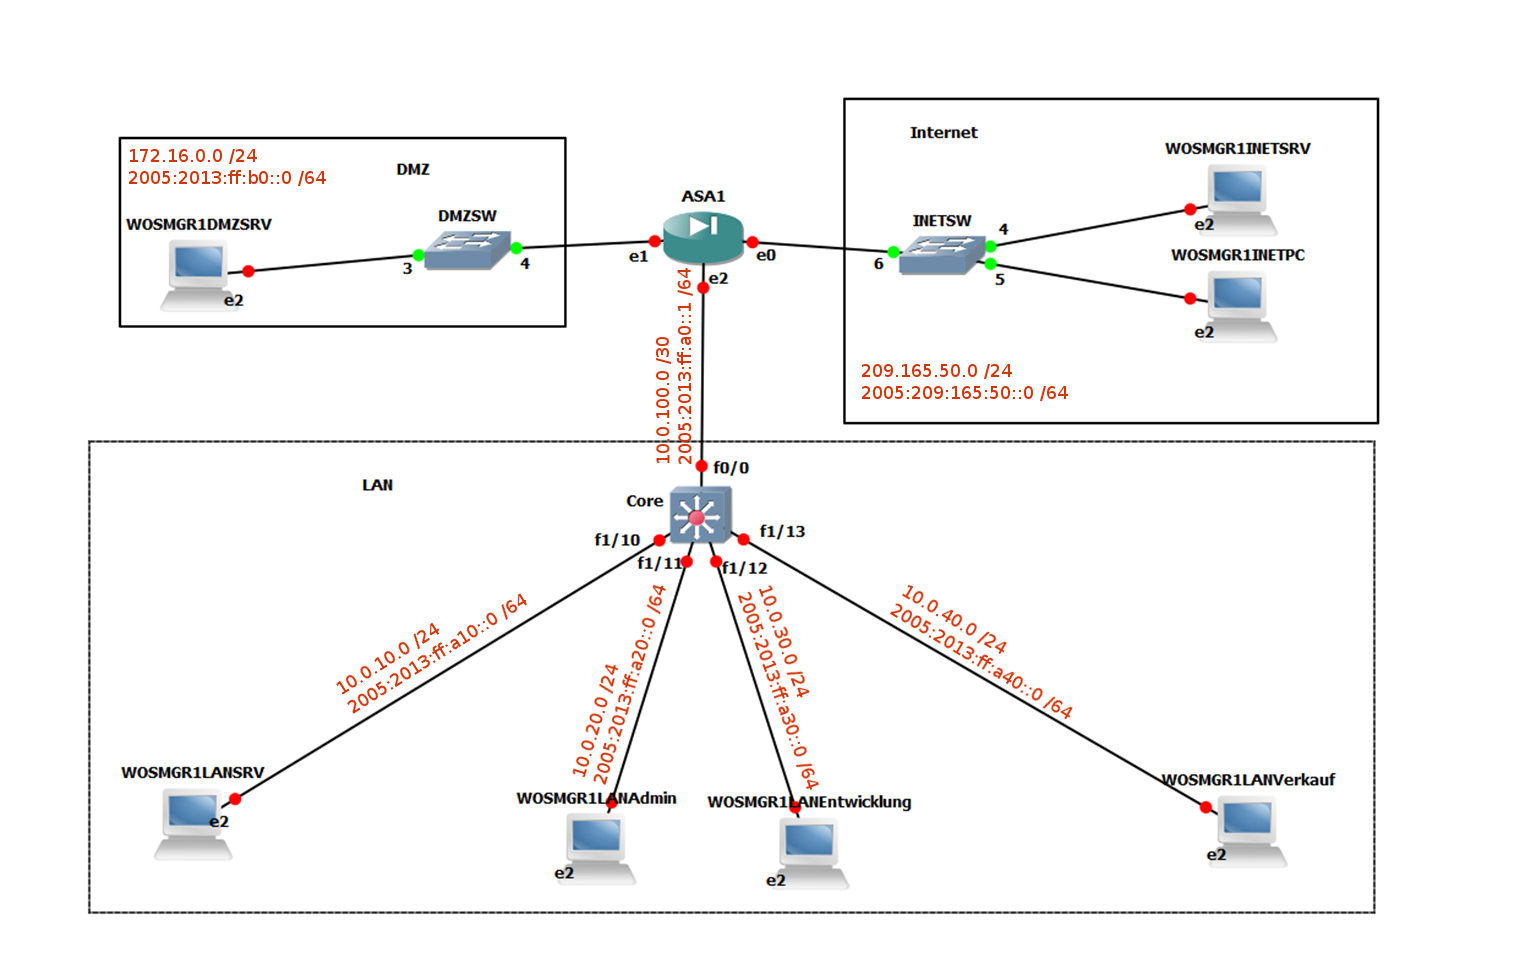
\includegraphics[width=1.0\textwidth]{Phase1/Netz_IP.png}
\caption{Netzwerk}
\label{fig:netzwerkdiagramm}
\end{figure}

\subsection{IP Dual-Stack Konzept}
\subsubsection{IPv4}
Wir unterscheiden zwischen drei verschiedenen Netzwerke. Das interne Netzwerk, das DMZ Netzwerk und das öffentliche Netzwerk. Wir verwenden für die DMZ und das interne Netzwerk verschiedene Netzwerkklassen um die Netze schnell unterscheiden zu können. Folgende IP-Adressierung und Maskierung werden wir verwenden.

\begin{longtable}{p{1.5cm}|p{4cm}|p{4cm}|p{3cm}}
	\textbf{VLAN} & \textbf{Funktion} & \textbf{IPv4 Range} & \textbf{IPv4 Gateway}\\
	\hline
	\endfirsthead
	\textbf{VLAN} & \textbf{Funktion} & \textbf{IPv4 Range} & \textbf{IPv4 Gateway}\\
	\hline
	\endhead
	\hline
	\multicolumn{2}{l}{\textit{Fortführung auf nächster Seite\ldots}} \\
	\endfoot
	\endlastfoot
	10 & Server & 10.0.10.0/24 & 10.0.10.1\\
	20 & Administratoren & 10.0.20.0/24 & 10.0.20.1\\
	30 & Entwicklung & 10.0.30.0/24 & 10.0.30.1\\
	40 & Verkauf & 10.0.40.0/24 & 10.0.40.1\\
	n/a & VPN Clients & 10.0.99.0/24 & n/a \\
	n/a & Infrastructure & 10.100.0.0/30 & n/a\\
	n/a & DMZ & 172.16.0.0/24 & 172.16.0.1\\
	n/a & WAN & 209.165.50.0/24 & 209.165.50.1
\end{longtable}

\subsubsection{IPv6}
Da die Hosts über das Internet direkt erreichbar sein sollen, werden wir globale IPv6 Adressen mit dem Site Prefix /64 verwenden.

\begin{longtable}{p{1.5cm}|p{4cm}|p{4cm}|p{4cm}}
	\textbf{VLAN} & \textbf{Funktion} & \textbf{IPv6 Range} & \textbf{IPv6 Gateway}\\
	\hline
	\endfirsthead
	\textbf{VLAN} & \textbf{Funktion} & \textbf{IPv6 Range} & \textbf{IPv6 Gateway}\\
	\hline
	\endhead
	\hline
	\multicolumn{2}{l}{\textit{Fortführung auf nächster Seite\ldots}} \\
	\endfoot
	\endlastfoot
	10 & Server & 2005:2013:FF:A10::/64 & 2005:2013:FF:A10::1\\
	20 & Administratoren & 2005:2013:FF:A20::/64 & 2005:2013:FF:A20::1\\
	30 & Entwicklung & 2005:2013:FF:A30::/64 & 2005:2013:FF:A30::1\\
	40 & Verkauf & 2005:2013:FF:A40::/64 & 2005:2013:FF:A40::1\\
	n/a & Infrastructure & 2005:2013:FF:A0::/64 & n/a\\
	n/a & DMZ & 2005:2013:FF:B0::/64 & 2005:2013:FF:B0::1/64\\
	n/a & WAN & 2005:209:165:50::/64 & 2005:209:165:50::1/64
\end{longtable}

\subsection{Adressvergabe an Clients}
\subsubsection{IPv4}
Die Clients stellen regulare DHCP-Anfragen. Um die Leases und Bereichsoptionen zentral und (einigermassen) angenehm über eine grafische Schnittstelle verwalten zu können, wird der Core-Router so konfiguriert, dass er die Anfragen an den internen Domänencontroller und DHCP-Server (INTSRV in VLAN10) weiterleitet. Der Router setzt dabei ein Flag in der Anfrage, welches es dem DHCP-Server erlaubt, festzustellen aus welchem Bereich die Anfrage kam. Nur so kann der Server beispielsweise einem Client aus dem Adminnetz eine IP aus dem Admin-Bereich zuweisen.

Der folgende Konfigurationsausschnitt zeigt die notwendigen Optionen (IPv6-betreffende Einstellungen entfernt):
\begin{lstlisting}
interface Vlan20
 description *** VLAN Admin ***
 ip address 10.0.20.1 255.255.255.0
 ip access-group ADMIN in
 ip helper-address 10.0.10.21
\end{lstlisting} 

Der Befehl \glqq{}ip helper address\grqq{} gibt an, wohin die DHCP-Anfrage weitergeleitet werden soll.

\subsubsection{IPv6}
Für die automatische Konfiguration der Client-Adressen für IPv6 kommen mehrere Möglichkeiten in Betracht:
\begin{description}
	\item[Autokonfiguration ohne DHCP] IPv6 sieht vor, dass Router Clients direkt das zu verwendende Netzwerkprefix angeben können und Clients sich dann mittels EUI-64 eine Adresse generieren. Da EUI-64 die (weltweit eindeutige) MAC-Adresse miteinbezieht, sind Adresskonflikte ausgeschlossen. Die Clients erfahren über Router-Advertisements, welche Netze sie über welche Router erreichen können.
		Leider ist keine Möglichkeit vorgesehen, den Clients mitzueteilen, welchen DNS-Server sie verwenden sollen. Somit kann dieser Ansatz alleine aktuell das Problem der Adressvergabe nicht abschliessend lösen.
	\item[DHCPv6 stateful] Diese Variante funktioniert sehr ähnlich wie die klassische DHCP Adressvergabe in IPv4-Netzen. Der Client fragt per Multicast (Broadcast-Adressen wurden in IPv6 abgeschafft) nach DHCP-Servern und \glqq{}bestellt\grqq{} sich eine Adresse. Die Angabe von weiteren Optionen, wie eine Liste der DNS-Server ist genau auf die selbe Art und weise möglich, wie dies bereits in IPv4-Netzen der Fall war. Eine Einschränkung ist bei unserer Konfiguration allerdings ins Gewicht gefallen: Der DHCP-Server kann den Clients keinen Default-Gateway angeben, eine entsprechende Option ist derzeit im Protokoll nicht vorgesehen.
	\item[DHCPv6 stateless] Diese Variante vereint die Stärken der beiden zuvor genannten Varianten der Adressvergabe. Die Konfiguration der IPv6-Adresse sowie des Gateways erfolgt per Router-Advertisements zwischen Router und Client. In der Antwort zur Router-Solicitation-Anfrage des Clients gibt der Router dem Client des Weiteren an, dass er weitere Informationen per DHCPv6 erfragen soll. Als Antwort auf die DHCP-Anfrage erhält der Client dann Optionen wie eine DNS-Serverliste oder den Domänennamen. Die Bezeichnung \glqq{}stateless\grqq{} rührt daher, dass der Server keine Informationen (Lease) zu den Clients speichern muss.
\end{description}

Auch dieser Ansatz soll mit einem Auszug der Schnittstellenkonfiguration verdeutlicht werden (IPv4 betreffende Konfigurationen entfernt):
\begin{lstlisting}
interface Vlan20
 description *** VLAN Admin ***
 ipv6 address 2005:2013:FF:A20::1/64
 ipv6 traffic-filter ADMINv6 in
 ipv6 nd other-config-flag
 ipv6 dhcp relay destination 2005:2013:FF:A10::21
\end{lstlisting}

Die Option \glqq{}ipv6 nd other-config-flag\grqq{} gibt an, dass der Router Clients darauf hinweisen soll, dass weitere Informationen über DHCPv6 erhalten werden können. Eine andere Einstellung hier wäre \glqq{}ipv6 nd managed-config-flag\grqq{} - dies würde den Client auffordern, auch seine IP-Adresse per DHCPv6 zu erfragen.

\glqq{}ipv6 dhcp relay destination\grqq{} gibt, analog zu der \glqq{}helper-adress\grqq{} bei IPv4, an, wohin DHCP-Anfragen weitergeleitet werden sollen.

Des Weiteren ist zu beachten, dass eintreffende \glqq{}Router-Solicitation\grqq{}-Anfragen der Clients nicht durch die ACL geblockt werden. Falls dies dennoch der Fall ist, erhält der Client die IPv6-Route erst nach einiger Zeit, da der Router von sich aus periodisch Router-Advertisement verschickt.

\subsection{Routing}
\subsubsection{Core Router}
Der Core Router hat nur default-routen konfiguriert. Sämtlicher Datenverkehr, der nicht in ein lokal angeschlossenes Netz soll, wird an die Firewall gesendet.

\begin{longtable}{p{4.5cm}|p{4cm}}
	\textbf{Zielnetz} & \textbf{Next Hop}\\
	\hline
	\endfirsthead
	\textbf{Zielnetz} & \textbf{Next Hop}\\
	\hline
	\endhead
	\hline
	\multicolumn{2}{l}{\textit{Fortführung auf nächster Seite\ldots}} \\
	\endfoot
	\endlastfoot
	0.0.0.0/0 & 10.100.0.2\\
	::/0 & 2005:2013:FF:A0::2
\end{longtable}

\subsubsection{Firewall}
Die default Route auf der Firewall würde normalerweise auf den Router des Service Providers zeigen. Da wir in der Simulation aber keinen solchen haben, werden keine default Routen konfiguriert. Die Firewall sendet somit nur den Verkehr für das interne Netzwerk an den Core Router.

\begin{longtable}{p{4.5cm}|p{4cm}}
	\textbf{Zielnetz} & \textbf{Next Hop}\\
	\hline
	\endfirsthead
	\textbf{Zielnetz} & \textbf{Next Hop}\\
	\hline
	\endhead
	\hline
	\multicolumn{2}{l}{\textit{Fortführung auf nächster Seite\ldots}} \\
	\endfoot
	\endlastfoot
	10.0.0.0/16 (Supernet) & 10.100.0.1\\
	2005:2013:FF:A10::/64 & 2005:2013:FF:A0::1\\
	2005:2013:FF:A20::/64 & 2005:2013:FF:A0::1\\
	2005:2013:FF:A30::/64 & 2005:2013:FF:A0::1\\
	2005:2013:FF:A40::/64 & 2005:2013:FF:A0::1
\end{longtable}

\subsection{NAT}
Network Address Translation wird für IPv4 verwendet um den internen Clients Zugriff ins Internet zu gewähren und um den Webserver in der DMZ vom Internet aus zugänglich zu machen. Für den Internetzugriff der Clients wird eine Port Address Translation (PAT) konfiguriert, damit nur eine Public IP-Adresse verwendet werden muss. Für den Webserver wird ein statisches NAT mit einer zusätzlichen Public IP-Adresse konfiguriert.

\begin{description}
	\item[Webserver] statisches NAT interne IP: 172.16.0.21 - öffentliche IP: 209.165.50.2
	\item[Interne Hosts] dynamisches NAT overload: interner Range: 10.0.0.0/16 - öffentliche IP 209.165.50.1 (Outside IF IP der Firewall)
\end{description}
Ausgenommen vom NAT ist die Verbindung vom Server Netzwerk (10.0.10.0/24) ins VPN Client Netzwerk (10.0.99.0/24) da sonst keine Verbindung von Remote Client zu Server erstellt werden kann.

\subsection{VTP}
Das VLAN Trunking Protokoll kommt in unserer Simulation nicht zu Einsatz, da GNS3 keine konfigurierbare Switches anbietet. Im Labor werden wir jedoch mit konfigurierbaren Switches arbeiten und VTP einsetzen. Der Core Router wird dabei der VTP Server sein und alle VLAN Informationen an die Switches verteilen.

\subsection{Spanning-Tree}
Spanning-Tree musste in der Simulation nicht berücksichtigt werden. Das Netzwerk ist sehr einfach aufgebaut und die Verbindung zwischen Core Router und Firewall benötigt keinen Spanning-Tree.

\subsection{VPN IPsec Remote Access}
Der Zugriff auf das interne Netzwerk für externe Mitarbeiter erfolgt über den IPsec VPN Client. Beim Zugriff unterscheiden wir zwischen Administratoren und Mitarbeiter. Der Zugriff als Mitarbeiter kann somit stärker eingeschränkt werden als ein Administrator. In der Simulation haben wir keine unterschiedlichen Zugriffsmöglichkeiten, die Firewall wurde aber für diesen Fall konfiguriert. Der Remote Access Zugang erfolgt über die IP 209.165.50.1 (Outside IF Firewall) und unterstützt nur IPv4.

\textbf{IKE Phase 1:}
\begin{itemize}
	\item{Authenzifizierung: Pre-shared}
	\item{Verschlüsselung AES 256-bit}
	\item{Hash SHA}
	\item{Schlüsselgenerierung Diffie-Hellman Group 2}
	\item{Gültigkeit Schlüsse 12h}
\end{itemize}

\textbf{IKE Phase 2 (Group-Policy):}
\begin{itemize}
	\item{Interne Gruppen (VPN\_ADMINISTRATOR \& VPN\_USERS\_GROUP)}
	\item{DNS-Server 10.0.10.21}
	\item{ACL 99: permit ip any 10.0.10.0 255.255.255.0 }
	\item{Split-Tunneling: 10.0.10.0/24}
	\item{Tunnel Protokol IKEv1 \& IKEv2}
	\item{Default Domain: wosm.com}
	\item{IP-Adressen Pools: VPN-ADMIN 10.0.99.0/25, VPN-USERS 10.0.99.128/25}
\end{itemize}

\subsection{Serverkonzept}
\begin{longtable}{p{3cm}|p{2.5cm}|p{2.3cm}|p{3.5cm}|p{3cm}}
	\textbf{Name} & \textbf{OS} & \textbf{IPv4} & \textbf{IPv6} & \textbf{Services}\\
	\hline
	\endfirsthead
	\textbf{Name} & \textbf{OS} & \textbf{IPv4} & \textbf{IPv6} & \textbf{Services}\\
	\hline
	\endhead
	\hline
	\multicolumn{2}{l}{\textit{Fortführung auf nächster Seite\ldots}} \\
	\endfoot
	\endlastfoot
	LANSRV & Windows Server 2008 R2 & 10.0.10.21 & 2005:2013:ff:a10::21 & AD, DNS, DHCP, Fileserver\\
	LANAdmin & Windows 7 & 10.0.20.21 & 2005:2013:ff:a20::21 & Client Admin\\
	LANEntwicklung & Windows 7 & 10.0.30.21 & 2005:2013:ff:a30::21 & Client Entwicklung\\
	LANVerkauf & Windows 7 & 10.0.40.21 & 2005:2013:ff:a40::21 & Client Verkauf\\
	DMZSRV & Windows Server 2008 R2	& 172.16.0.21 & 2005:2013:ff:b0::21	& HTTP, HTTPS, FTP\\
	INETSRV	& Windows Server 2008 R2 & 209.165.50.21 & 2005:209:165:50::21 & HTTP, HTTPS, FTP\\
	INETPC & Windows 7 & 209.165.50.22 & 2005:209:165:50::22 & Client Extern\\
\end{longtable}


\newpage
\section{Sicherheit}
\subsection{Konzept}
Um die Sicherheit unseres Netzes zu gewähtleisten, haben wir uns entschieden, verschiedene Sicherheitsstufen zu definieren. Dabei verfolgen wir eine High Security Strategie. Die höchste Sicherheitsstufe 'Stufe 1' gilt für die normalen User. Die zweite Sicherheitsstufe 'Stufe 2' gilt für die Server. Die dritte Sicherheitsstufe 'Stufe 3' gilt für die Administratoren.

Bei der Sicherheitsstufe Stufe 1 wird nur das nötigste zugelassen und alles andere blockiert. Die User dürfen über Ports 80 und 443 im Internet surfen, sowie FTP Verbindungen über Port 21 und 20 öffnen. Zudem werden eingehende DHCP Anfragen über den Port UDP 68 zugelassen.

Bei der Sicherheitsstufe Stufe 2 wird alles zugelassen, was die Server benötigen. Dabei wird aus den VLANs 20, 30 und 40 alles zugelassen. Aus der DMZ wird nur der Port 389 für LDAP zugelassen.

Bei der Sicherheitsstufe Stufe 3 wird zusätzlich zu den in Stufe 1 zugelassenen Ports noch der Port 22 im internen Netz und in die DMZ zur Verwaltung der Netzwerkgeräte zugelassen. Zudem ist beim Internetzugang für die Administratoren alles offen.

Die definierten Sicherheitsstufen wurden mithilfe verschiedener ACLs umgesetzt. Die definierten Regeln (Auflistung oben nicht abschliessend) der ACL's sind im folgenden Kapitel ersichtlich.

Die ACLs werden möglichst nahe an der Quelle angewendet. Somit sind alle ACLs welche den Zugriff der verschiedenen internen VLANs in irgend ein anderes Netz regeln auf dem Core Switch auf den VLAN-Interfaces in Richtung \emph{in} angewendet. Alle ACLs die den Zugriff in die DMZ, resp. von der DMZ in ein anderes Netz regeln werden auf der ASA angewendet. Alle ACLs die den eingehenden Traffic aus dem Internet regeln sind ebenfalls auf der ASA angewendet.

Mit einer Stateful Firewall sinkt einerseits der Konfigurationsaufwand und gleichzeitig kann eine höhere Sicherheit erreicht werden. Da wir eine High Security Strategie verfolgen, ist die Stateful Variante besser geeignet für unsere Zwecke.

\subsection{Firewall}
\subsubsection{ACL auf Core-Router}
Auf diesem Router sind ACL für alle angeschlossenen VLANs definiert. Die folgende Tabelle liefert einen Überblick, die kompletten ACL sind im Anhang dieser Dokumentation zu finden.
\begin{longtable}{p{2.5cm}|p{3.5cm}|p{7cm}}
	\textbf{Name} & \textbf{Interface/Richtung} & \textbf{Anmerkung}\\
	\hline
	\endfirsthead
	\textbf{Name} & \textbf{Interface/Richtung} & \textbf{Anmerkung}\\
	\hline
	\endhead
	\hline
	\multicolumn{2}{l}{\textit{Fortführung auf nächster Seite\ldots}} \\
	\endfoot
	\endlastfoot
	INTSRV & VLAN 10 / in & Reglementiert IPv4 Traffic, der aus dem Servernetz verschickt werden darf.\\
	INTSRVv6 & VLAN 10 / in & Reglementiert IPv6 Traffic, der aus dem Servernetz verschickt werden darf.\\
	ADMIN & VLAN 20 / in & Reglementiert IPv4 Traffic, der aus dem Adminnetz verschickt werden darf.\\
	ADMINv6 & VLAN 20 / in & Reglementiert IPv6 Traffic, der aus dem Adminnetz verschickt werden darf.\\
	DEV & VLAN 30 / in & Reglementiert IPv4 Traffic, der aus dem Entwicklungsnetz verschickt werden darf.\\
	DEVv6 & VLAN 30 / in & Reglementiert IPv6 Traffic, der aus dem Entwicklungsnetz verschickt werden darf.\\
	VERKAUF & VLAN 40 / in & Reglementiert IPv4 Traffic, der aus dem Verkaufsnetz verschickt werden darf.\\
	VERKAUFv6 & VLAN 40 / in & Reglementiert IPv6 Traffic, der aus dem Verkaufsnetz verschickt werden darf.\\
\end{longtable}

\subsubsection{ACL auf ASA}
Auf der Firewall wurden jeweils 3 Access Lists definiert. Diese werden auf den jeweiligen Interfaces angewendet. Die kompletten Access-lists sind im Anhang zu finden.

\begin{longtable}{p{2.5cm}|p{3.5cm}|p{7cm}}
	\textbf{Name} & \textbf{Interface/Richtung} & \textbf{Anmerkung}\\
	\hline
	\endfirsthead
	\textbf{Name} & \textbf{Interface/Richtung} & \textbf{Anmerkung}\\
	\hline
	\endhead
	\hline
	\multicolumn{2}{l}{\textit{Fortführung auf nächster Seite\ldots}} \\
	\endfoot
	\endlastfoot
	dmz\_in & dmz / in & IPv4 Traffic, der aus dem DMZ-Netzwerk verschickt werden darf.\\
	dmz\_in\_v6 & dmz / in & IPv6 Traffic, der aus dem DMZ-Netzwerk verschickt werden darf.\\
	inside\_in  & inside / in & IPv4 Traffic, der aus dem internen Netzwerk verschickt werden darf.\\
	inside\_in\_v6 & inside / in & IPv6 Traffic, der aus dem internen Netzwerk verschickt werden darf.\\
	outside\_in & outside / in & IPv4 Traffic, der aus dem Internet verschickt werden darf.\\
	outside\_in\_v6 & outside / in & IPv6 Traffic, der aus dem Internet verschickt werden darf.\\
\end{longtable}

\newpage
\section{Bedrohungsmodell}
\subsection{TCP DoS (SYN-Flooding)}
\subsubsection{Bedrohung}
Beim TCP 3-Way Handshake wird zuerst eine Anfrage an einen Server gesendet, indem ein TCP Paket mit dem Flag SYN verschickt wird. Der Server als Empfänger dieses TCP SYN Pakets verarbeitet dieses und sendet ein TCP Paket mit den Falgs SYN und ACK zurück. Er merkt sich dabei in einer SYN-Liste, mit wem er ein 3-Way Handshake begonnen hat. Wenn derInitiator der Verbindung das TCP Paket mit den Flags SYN und ACK empfängt, verarbeitet er dieses und sendet zur Bestätigung ein Paket mit dem Flag ACK. Sobald der Server das Packet mit dem Flag ACK erhalten hat, wird der Eintrag in der SYN-Liste gelöscht.

Ein Angreifer sendet 100 SYN-Anfragen pro Sekunde an einen bestimmten Server. Dabei setzt er eine andere Source IP Adresse, sodass die Antwort nicht zum Angreifer kommt. Da sich der Server merkt, mit wem er einen 3-Way Handshake begonnen, diese aber nicht abschliessen kann, da nie eine Bestätigung mit dem Flag ACK eintrifft, wird der Arbeitsspeicher des Server gefüllt. Sobald der Speicher gefüllt ist, kann dieser keine weiteren Verbindungen mehr aufnehmen oder stürtzt ab.

\subsubsection{Gegenmassnahme}
Um einen Webserver vor diesem Angriff zu schützen, kann auf der ASA eine Policy erstellt werden, welche die maximale Anzahl Verbindungen und halb offener Verbindungen limitiert. Zudem können Timeouts gesetzt werden, wie lange eine Verbindung in welchem Status sein darf (halb offen, offen, halb geschlossen).

Auf einem normalen Router kann mit SYN-Cookies oder SYN-Cache gearbeitet werden. Dadurch sind die Server hinter der ASA vor SYN-Flooging Attacken geschützt.

\subsection{IP spoofing}
\subsubsection{Bedrohung}
Ein Anfreifer sendet viele Anfragen an einen Server mit einer falschen Absender IP (z.B: 10.0.1.19). Dadurch wird der Server die Antworten zu den Anfragen an einen Client (10.0.1.19) senden. Der Server, sowie der Client wird dadurch ausgelastet.
\subsubsection{Gegenmassnahme}
Um sich gegen IP spoofing zu schützen, kann eine Überprüfung des 'Reverse-Path' aktiviert werden. So wird überprüft, ob die eingetragene Absenderadresse mit der effektiven Absenderadresse übereinstimmt.

\subsection{ICMP ‘smurf attack’: Denial of Service}
\subsubsection{Bedrohung}
Ein Angreifer sendet ein ICMP Packet mit einer Echo-Anfrage an eine oder mehrere Broadcasts und verwendet als Absenderadresse die IP Adresse des Servers (Opfer). Die Broadcastanfrage wird an alle Hosts in betroffenen Netz weitergeleitet. Die Hosts senden daraufhin ein die Echo-Antwort an den Server (Opfer). Der Server empfängt nun so viele Echo Antworten dass der Server nicht mehr reagiert und abstürtzt.
\subsubsection{Gegenmassnahme}
Um diese Attacke abzuwehren, kann ICMP blockiert werden. So ist sichergestellt, dass keine Echo Antworten den Server erreichen.

\subsection{Viren / Würmer / Trojaner}
\subsubsection{Bedrohung}
Programme, welche vertrauliche Informationen stehlen, Schaden auf den Hosts anrichten oder die Kontrolle über einen Host übernehmen und ihn für eigene Zwecke einsetzen. Zudem können diese Programme zum Beispiel als SMTP Relay fungieren und SPAM Nachrichten versenden, wodurch die Public IP auf einer Blackliste gelistet werden kann.
\subsubsection{Gegenmassnahme}
Um sich gegen Viren, Würmer und Trojaner zu schützen, muss ein Anti-Virenprogramm auf jedem Host installiert werden.

\subsection{DNS Cache poisoning}
\subsubsection{Bedrohung}
Ein Angreifer bringt bei einem DNS Server gefälschte Daten in den Cache. Wenn nun ein Benutzer auf diese Daten zugreift, wird dieser auf manipulierte Seiten weitergeleitet. Der Angreifer kann nun mit Phishing Daten des Benutzer stehlen.

\subsubsection{Gegenmassnahme}
Der beste Schutz gegen diesen Angriff ist der Einsatz von DNSSEC, welcher mit Authentifizierung und Integrität arbeitet.
\subsection{Phishing}
\subsubsection{Bedrohung}
Beim Phishing versucht ein Angreifer durch gefälschte Websiten, SPAM Mails oder andere Methoden an Daten eines Internet-Benutzer zu gelangen. So kann ein Angreifer an Kreditkarteninformationen oder weitere Daten kommen und einen erheblichen finanziellen Schaden anrichten.
\subsubsection{Gegenmassnahme}
Leider gibt es gegen diese Attacke keine effektive Schutzmassnahme. Um sich möglichst gut gegen diese Attacke zu schützen, müssen die Benutzer geschult werden. Zudem kann ein SPAM Filter Mails von potentiellen Angreifern löschen oder markieren, sodass sich der Benutzer dem Risiko bewusst ist.

\subsection{MAC flooding}
\subsubsection{Bedrohung}
Ein Angreifer sendet viele ARP Antworten. Dabei setzt er immer eine andere MAC Adresse. Wenn die Index Tabelle des Switches voll ist, schaltet dieser in den Hub Modus um und sendet alle Packete jedem angeschlossenen Gerät. Nun kann der Angreifer jegliche Kommunikation über diesen Switch mithören. 
\subsubsection{Gegenmassnahme}
Um sich gegen diese Attacke zu schützen, kann auf dem Switch definiert werden, dass er ausschalten soll, wenn die Index Tabelle voll ist. Dadurch ist zwar ein Unterbruch im Netz vorhanden, aber der Angreifer kann den Datenverkehr nicht mithören.

Eine noch besserer Schutz ist, wenn die Port Security auf dem Switch aktiviert und konfiguriert wird. Dadurch hat kein Angreifer die Möglichkeit die Index Tabelle des Switches zu füllen.

\subsection{ARP spoofing}
\subsubsection{Bedrohung}
Ein Angreifer sendet ARP Antworten mit den IP Adressen der Opfer und seiner eigenen MAC Adresse. Der Switch merkt sich nun dass die IP Adressen zur MAC Adresse des Angreifers gehören. Wenn nun ein Opfer ein Paket sendet, wird dieses vom Switch zum Angreifer weitergeleitet. Der Angreifer hat nun Einblick in die Daten, kann diese allenfalls verändern und leitet dieses schliesslich weiter zum effektiven Ziel, sodass niemand etwas davon mitbekommt.
\subsubsection{Gegenmassnahme}
Um sich gegen diese Attacke zu schützen, kann die Port Security auf dem Switch aktiviert werden, dadurch hat ein potentieller Anfreifer gar keine Möglichkeit sich ins interne Netz einzubinden.

\subsection{Rogue DHCP}
\subsubsection{Bedrohung}
Eine Person mit Zugriff auf ein Netzwerkkabel im internen Netz verbindet einen zusätzlichen, nicht autorisierten DHCP Server. Wenn der zusätzliche DHCP Sever schnellere Antwortzeiten hat als der offizielle DHCP Server, erhalten die Clients nun eine IP des nicht autorisierten DHCP Server, wodurch diese nicht mehr auf die interne Infrastruktur zugreiffen können.
\subsubsection{Gegenmassnahme}
Um dies zu verhindern, kann der Port 68 für DHCP Antworten blockiert werden (ausser vom offiziellen DHCP Server). Dadurch ist sichergestellt, dass kein zusätzlicher DHCP Server IP Adressen im interne Netz verteilen kann.

\subsection{Überblick}
\begin{longtable}{p{1.4cm}|p{3.9cm}|p{2.6cm}|p{4cm}|p{2cm}}
	\textbf{Rang} & \textbf{Wahrscheinlichkeit} & \textbf{Schweregrad} & \textbf{Bedrohung} & \textbf{Schutz umgesetzt}\\
	\hline
	\endfirsthead
	\textbf{Ranking} & \textbf{Eintrittswahrscheinlichkeit} & \textbf{Schweregrad} & \textbf{Bedrohung} & \textbf{Schutz umgesetzt}\\
	\hline
	\endhead
	\hline
	\multicolumn{2}{l}{\textit{Fortführung auf nächster Seite\ldots}} \\
	\endfoot
	\endlastfoot
	1 & hoch & hoch & ICMP ‘smurf attack’: Denial of Service & ja\\
	2 & hoch & mittel & Viren / Würmer / Trojaner & nein\\
	3 & mittel & hoch & TCP DoS (SYN-Flooding) & ja\\
	4 & mittel & hoch & DNS Cache poisoning & nein\\
	5 & hoch & niedrig & Phishing & nein\\
	6 & niedrig & hoch & Rogue DHCP & ja\\
	7 & niedrig & mittel & IP spoofing & ja\\
	8 & niedrig & mittel & MAC flooding & nein\\
	9 & niedrig & mittel & ARP spoofing & nein\\
\end{longtable}

\subsection{Verteidigung gegen Attacken}
\subsubsection{ICMP ‘smurf attack’: Denial of Service}
\begin{lstlisting}
object-group service inet2dmzsrv_TCPPorts tcp
 port-object eq www
 port-object eq https
 port-object eq ftp-data
 port-object eq ftp
 port-object range 48999 49999
!
access-list outside_in remark wan-dmzsrv
access-list outside_in extended permit tcp any host 172.16.0.21 object-group inet2dmzsrv_TCPPorts
access-list outside_in extended deny ip any any log
!
icmp deny any outside
\end{lstlisting}

\subsubsection{TCP DoS (SYN-Flooding)}
Folgende Policy Map schützt gegen SYN-Flooding:
\begin{lstlisting}
policy-map tcpmap
 class tcp_syn
  set connection conn-max 100 embryonic-conn-max 100 per-client-max 10 per-client-embryonic-max 10
  set connection timeout embryonic 0:00:45 half-closed 0:05:00 idle 1:00:00
!
class-map tcp_syn
 match any
\end{lstlisting}

\subsubsection{IP spoofing}
Folgender Befehl schützt gegen IP spoofing:
\begin{lstlisting}
ip verify reverse-path interface outside
\end{lstlisting}

\subsubsection{DHCP IPv4}
Die ACL für die internen Client-VLANs verhindert das Versenden einer Antwort auf eine DHCP-Anfrage. Um die Beantwortung aus dem Servernetz zu erlauben wurden die folgenden Regeln angewendet:

\begin{lstlisting}
permit udp 10.0.10.0 0.0.0.255 eq 67 10.0.20.1 0.0.0.0 eq 67
permit udp 10.0.10.0 0.0.0.255 eq 67 10.0.30.1 0.0.0.0 eq 67
permit udp 10.0.10.0 0.0.0.255 eq 67 10.0.40.1 0.0.0.0 eq 67
\end{lstlisting}

Bei der Situation, einen DHCP-Server innerhalb eines Client VLANs daran zu hindern, anderen Clients im selben VLAN eine Adresse zuzuteilen, müsste eine ACL auch auf den Switches angewendet werden (Richtung: in), welche den Datenverkehr über UDP von Quellport 67 an Zielport 68 nicht erlaubt.

\subsubsection{Autoconfiguration IPv6}
Bei IPv6 ist dieses Problem etwas anders zu handhaben. Es muss verhindert werden, dass Clients Router-Advertisements verschicken können. Dies kann durch einen ACL-Eintrag der folgenden Art umgesetzt werden (die ACL müsste in Richtung \emph{in} auf dem zu den Clients führenden IFs angewendet werden):

\begin{lstlisting}
deny icmp any any router-advertisement
\end{lstlisting}

Analog IPv4 muss ebenfalls der Traffic von UDP Quellport 547 an den Zielport 546 aus den Client-Netzen unterbunden werden.

\newpage
\section{Probleme mit Simulator}
Bei unserer Arbeit mit dem Simulator sind einige Probleme aufgetreten, für welche wir keine Lösung gefunden haben.

\subsection{Ressourcen lokaler Rechner}
Wenn im Simulator VMs über VirtualBox eingebunden werden und der lokale Rechner nichts genügend oder nur knapp genügend RAM hat, kann es vorkommen, dass  die komplette Simulation abstürtzt. Die komplette Simulation konnte daher nur auf den Rechnern ausgeführt werden mit mindestens 8GB RAM.
\subsection{SSL VPN Image}
In der Simulation kann grundsätzlich das zu verwendende Image für ein Netzwerkgerät gewählt und eingespielt werden. Bei der ASA konnte jedoch das SSL VPN Image nicht eingespielt werden. Das Upload des Images auf die ASA war nicht möglich. Bei jedem Versuch das Image einzuspielen erschien der Fehler 'unspecified error' bei ca. 60\% des Uploads.
\subsection{ASA und Linux}
Die simulierte ASA konnte auf Windows korrekt gestartet werden. Unter Linux wurde der Bootvorgang gestartet, aber nie richtig abgeschlossen (Crash). Eine komplette Simulation unseres Netzes war mit Linux daher nicht möglich.
\subsection{Anbindung VirtualBox}
Die virtuellen Maschinen müssen aus dem Simulator gestartet werden, damit diese auch im Simulator verwedent werden können. Falls nun eine VM über das Betriebssystem abgestellt wird, erkennt der Simulator nicht, dass die VM nicht mehr läuft. Diese muss im Simulator anschliessend noch manuell beendet werden.\\
Die VM kann aber auch über den Simulator abgestellt werden. Bei einem Shutdown über den Simulator wird die VM jedoch sofort beendet, ohne korrekten Shutdown des Betriebssystems.

\newpage
\section{Lab}
\subsection{Berechtigungskonzept}
Das Berechtigungskonzept ist in der Aufgabenstellung vorgegeben. Da dies jedoch unterschiedlich interpretiert werden kann, beschreiben wir dies noch einmal kurz.

\begin{itemize}
\item{Jeder User hat ein eigenes persönliches Laufwerk}
\item{Jeder User hat Zugriff auf die Allgemeinen Dateien seiner Abteilung}
\item{Jeder Abteilungsleiter hat Zugriff auf alle Dateien seiner Abteilung inkl. persönlicher Laufwerke seiner Mitarbeiter}
\item{Die Administratoren haben Zugriff auf alle Daten der Firma}
\end{itemize}
\subsection{Active Directory und Fileserver}
Um das Berechtigungskonzept umzusetzen und dem Administrator die Verwaltung zu vereinfachen haben wir uns für eine Struktur entschieden die wie folgt aussieht:
\begin{itemize}
\item[-]{wosm.com}
\begin{itemize}
\item[-]{MyBusiness}
\begin{itemize}
\item[-]{Admin}
\item[-]{Entwicklung}
\item[-]{Verkauf}
\end{itemize}
\end{itemize}
\end{itemize}
Um die firmenspezifischen Einrträge zu verwalten wurde die OU 'MyBusiness' erstellt. Dies hilft uns den Überblick zu bewahren und schützt vor Fehlmanipulationen, da die Default Microsoft Berechtigungsgruppen und User klar von den firmenspezifischen Einträgen getrennt sind.

Zudem wurde für jede Abteilung eine eigene OU erstellt, in welcher nun die Abteilungsspezifischen Berechtigungsgruppen und Benutzer erstellt werden.

Für jede Abteilung haben wir eine Berechtigunsgruppe [Abteilung] und [Abteilung]\_Leitung erstellt, sowie die Benutzer für den Abteilungsleiter und die Mitarbeiter. Am Beispiel Verkauf sieht dies wie folgt aus:
\begin{itemize}
\item[-]{Verkauf}
\begin{itemize}
\item[+]{Verkauf}
\item[+]{Verkauf\_Leitung}
\item[°]{User40}
\item[°]{User41}
\item[°]{User42}
\end{itemize}
\end{itemize}
In der Gruppe 'Verkauf\_Leitung' ist der Benutzer 'User40'. In der Gruppe 'Verkauf' ist die Gruppe 'Verkauf\_Leitung' sowie die Benutzer 'User41' und 'User42'.

Auf dem Fileserver wurde für jede Abteilung ein eigener Ordner erstellt, auf welchen nur die jeweilige Abteilung sowie die Administratoren Zugriff haben. Zudem werden alle persönlichen Ordner auf dem Fileserver (Ordner wird direkt im AD verwaltet und automatisch erstellt, da es als Home-Laufwerk angegeben wird) erzeugt. Die Struktur sowie die Berechtigungen sehen wie folgt aus (Ordner : Berechtigungsgruppe 1, Berechtigungsgruppe 2, ...) :
\begin{itemize}
\item[-]{Verkauf : Verkauf\_Leitung, Administratoren}
\begin{itemize}
\item[-]{Allgemein : Verkauf\_Leitung, Verkauf, Administratoren}
\item[-]{User40 : Verkauf\_Leitung, User40, Administratoren}
\item[-]{User41 : Verkauf\_Leitung, User41, Administratoren}
\item[-]{User42 : Verkauf\_Leitung, User42, Administratoren}
\end{itemize}
\end{itemize}
Damit alle Mitarbeiter aus der Abteilung Verkauf auf ihre Ordner zugreifen können, wurde der Order 'Verkauf' für die Gruppe 'Verkauf' und 'Administratoren' freigegeben.

Die Struktur, sowie die Berechtigungen sehen bei den anderen Abteilungen gleich aus, jedoch mit deren Berechtigungsgruppen.

Die Verwaltung wurde durch die oben definierte Struktur soweit vereinfacht, dass bei der Erstellung eines weiteren Benutzers ein bestehender Benutzer kopiert werden kann und lediglich das Home-Laufwerk angegeben werden muss.
\subsection{Logonscript}
Das persönliche Laufwerk wird automatisch als Z: verbunden, da dies im Active Directory als Home-Laufwerk angegeben wurde.

Damit alle Benutzer auf die für sie relevanten Dateien Zugriff haben, haben wir ein Logonscript erstellt, welches überprüft in welcher Berechtigungsgruppe ein Benutzer ist und dementsprechend ein Netzlaufwerk verknüpft.

Das Logonscript sieht folgendermassen aus:
\lstinputlisting{Phase2/logonscript.bat}

\subsection{Radius}
Damit für den VPN Zugang die Active Directory Benutzer verwendet werden können, haben wir auf dem LAN Server ein Radius Dienst installiert. Microsoft nennt diesen Dienst Internet Authentication Service (IAS), welcher mit der Rolle Netzwerkrichtlinien- und Zugriffsdienste installiert wird. Um die Benutzerabfrage zu ermöglichen muss die ASA Firewall als Client erfasst werden. Dazu ist lediglich die IP-Adresse des Clients (ASA) und ein gemeinsamer Schlüssel für die Kommunikation notwendig. Die Verbindungsbedingungen können anhand einer Netzwerkrichtlinie eingestellt werden. Diese bietet viele Konfigurationsmöglichkeiten wie Verschlüsselungsmethode, Zugriffszeit usw. Unsere Einschränkung bezieht sich lediglich auf
die Benutzergruppen. Dies bedeutet nur AD Benutzer, welche in den Gruppen Admin, Admin\_Leitung, Verkauf und Verkauf\_Leitung sind, können sich authentifizieren und somit eine gesicherte Verbindung herstellen.

\subsection{Tunnelling mit Tinc}
\subsubsection{Grund für diese Lösung}
In Phase 2 stehen die Netzwerkkomponenten (Layer 3 Switch, ASA) im Lab und die VMs werden auf einer VMware Virtualisierungsumgebung betrieben. Da es auf Grund von Einschränkungen bei der Vernetzung der beiden Räume nicht möglich ist, die Leitung als Trunk zu betreiben, mussten wir uns nach einer Umgehung dieser Einschränkung umsehen:

\begin{description}
	\item[Nur logische Trennung der Netze] bei dieser Variante wären alle VLANs ungetaggt über die Verbindung zwischen Lab und VMware-Umgebung geführt worden. Da sich die Rechner in unterschiedlichen IP-Netzen befinden wären nur geringe Einschränkungen entstanden. DHCP mit unterschiedlichen IP-Ranges für die verschiedenen VLANs hätte mit dieser Variante aber nicht ermöglicht werden können, da der Server die DHCP-Anfragen der Clients (Broadcast) direkt beantwortet hätte.
	Des Weiteren wäre es notwendig gewesen, die Konfiguration des Layer 3 Switches 
	\item[Nachfrage bei Herrn Schindler] Ergab leider lediglich, dass es nicht möglich sei, die vorhandene Verbindung als Trunk zu realisieren.
	\item[Tunnelling der unterschiedlichen Netze] Bei dieser Variante ist es unter Verwendung eines zusätzlichen Switches möglich, die bestehende Konfiguration des Layer 3 Switches weiterhin zu verwenden. Ebenfalls kann DHCP ohne Einschränkungen betrieben werden.
\end{description}

Aufgrund der Vorteile der Tunnelling Lösung gegenüber der nur logischen Trennung haben wir uns dazu entschieden, die Netze zu tunneln.

\subsubsection{Überblick}
Tinc ermöglicht es, Netze über UDP/IP-Verbindungen zu tunneln als wären sie über einen Switch verbunden. Dadurch können Geräte im selben VLAN (z.B. das vlan10-Interface des L3 Switches und die VM für den internen Server) miteinander kommunizieren als wären sie direkt auf Layer 2 miteinander verbunden. Abbildung \ref{fig:tinc} zeigt exemplarisch die Konfiguration für den Tunnel von VLAN 10.

\begin{figure}[H]
\centering
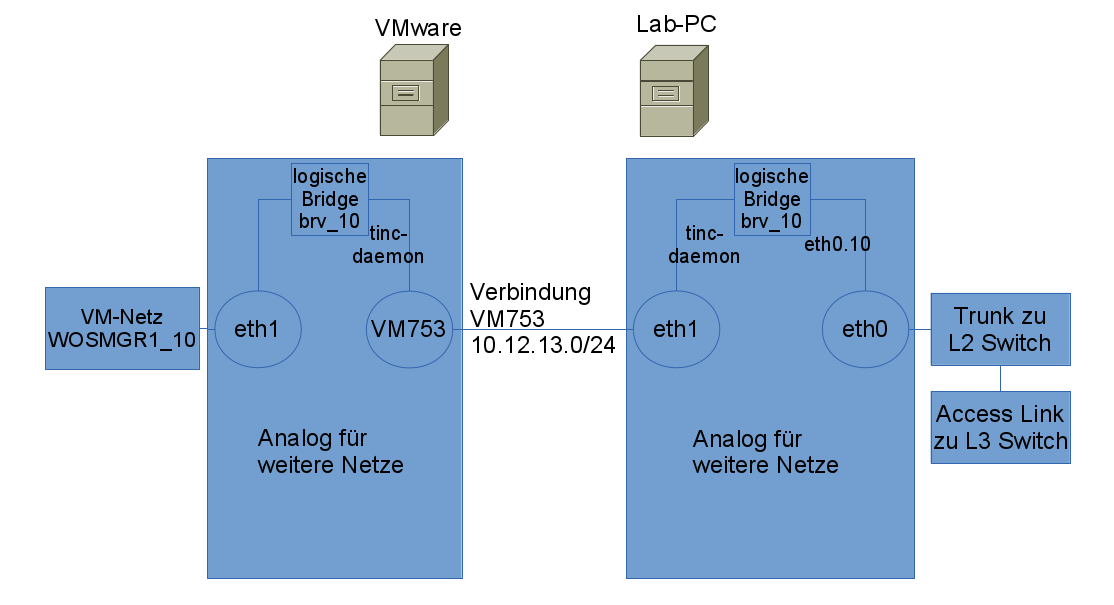
\includegraphics[width=1.0\textwidth]{Phase2/tinc_netz.png}
\caption{Tinc Funktionsweise / Aufbau}
\label{fig:tinc}
\end{figure}

\subsubsection{Konfiguration auf VMware-Umgebung}
Die VM, welche auf VMware-Seite die Tinc-Tunnels terminiert wird als einzige in das vorbereitete VM753-Netz verbunden. Pro VLAN wird auf dem virtuellen VMware-Switch eine zusätzliche Portgruppe definiert. In diese Portgruppe werden dann sowohl die VMs des jeweiligen Netzes als auch ein Interface der Tunnel-VM konfiguriert. Einen Auszug der Netzwerkkonfiguration zeigen die Abbildungen \ref{fig:tinc-esx-overview} und \ref{fig:tinc-esx-tunvm}.

\begin{figure}[H]
\centering
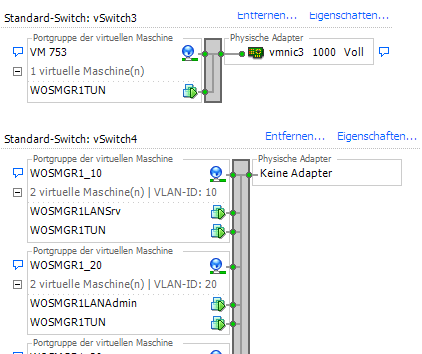
\includegraphics[width=0.7\textwidth]{Phase2/tinc_esx_netz.png}
\caption{Netze auf VMware-Umgebung}
\label{fig:tinc-esx-overview}
\end{figure}

\begin{figure}[H]
\centering
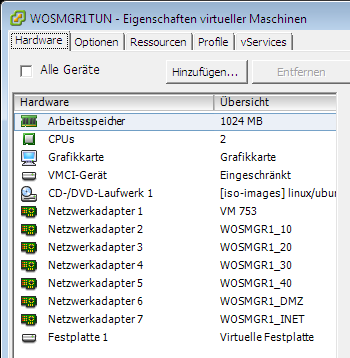
\includegraphics[width=0.5\textwidth]{Phase2/tinc_wosmgr1tun.png}
\caption{Netzwerkkonfiguration Tunnel-VM}
\label{fig:tinc-esx-tunvm}
\end{figure}

\subsubsection{Einrichtung der Tinc-Daemons}
Tinc braucht für das Tunnelling einer Verbindung eine Software-Bridge, an die das erstellte Pseudo-Device angeschlossen werden kann. Die Bridge kann unter Linux folgendermassen erstellt werden (Beispiel: VLAN 10 auf der Tunnel-VM auf VMware):

\begin{lstlisting}
brctl addbr brv_10
ifconfig eth1 0.0.0.0
ifconfig brv_10 up
brctl addif brv_10 eth1
ifconfig eth1 up
\end{lstlisting}

Im Konfigurationsverzeichnis des Tunnels (in diesem Beispiel unter /etc/tinc/bridge\_10/) ist danach eine Datei tinc.conf mit folgenden Inhalt zu erstellen:

\begin{lstlisting}
BindToAddress 10.12.13.1 10010
Name = vlan10_esx
Mode = switch
ConnectTo = vlan10_lab
\end{lstlisting}

Der Eintrag hinter \emph{ConnectTo} bezieht sich dabei auf Files, die unter /etc/tinc/bridge\_10/hosts/ abzulegen sind. In diesen Files sind auch RSA-Keys enthalten, der Befehl \emph{tincd -K} kann benutzt werden um RSA-Schlüsselpaare für Tinc zu erzeugen. Die Host-Dateien sehen folgendermassen aus (Beispiel: vlan10\_esx):

\begin{lstlisting}
Address = 10.12.13.1 10010
-----BEGIN RSA PUBLIC KEY-----
MIIBCgKCAQEAwgQKXRxDjyjL89+4qe3YeFYAFtL5ugFkZS8K/Y9h6HK7dkCZcATl
HM1FS+2UuSbgMd8U7zMd33W0KMat5iZfj/08uQO9cTyx/TibbP7HXpIFRJ/BeB5p
sKvR/SjcWRFPHHC+LIUKLbDkx+SvMaEo/PfswVFFw2Xp8MIYHGH4/ow9cqJjeABH
d6KOwUsDeVF/3pgcuoXL2hw1Iem3SRmQds2siRYkn1UyYWmQ2zHXeTdjym30KDMh
s0Nz8QjJrRFQzADjugAiyktviuI7sqwnjbEIsAlPDVU76ObBN/vPTavH9r8nDEF8
iQSVSfXIob8GThsnikVhUTBElAA17DLEaQIDAQAB
-----END RSA PUBLIC KEY-----
\end{lstlisting}

Tinc braucht des Weiteren ein \emph{tinc-ifup} Script, welches nach der Initialisierung des Tunnel-Interfaces ausgeführt wird. Das folgende Beispielt fügt das Tunnel-Interface (\$INTERFACE) der Bridge brv\_10 hinzu:

\begin{lstlisting}
#!/bin/sh
ifconfig $INTERFACE 0.0.0.0
brctl addif brv_10 $INTERFACE
ifconfig $INTERFACE up
\end{lstlisting}

Sind alle diese Vorbereitungen getroffen kann der Tunnel mit dem Befehl \emph{tincd -n bridge\_10} gestartet werden. \emph{bridge\_10} bezieht sich dabei auf das Konfigurationsverzeichnis unterhalb von \emph{/etc/tinc/}.

\subsubsection{VLAN-Subinterfaces unter Linux}
Die zuvor beschriebenen Punkte reichen für die VM unter VMware aus. Für die Installation im Lab ist es hingegen (aufgrund der begrenzten Anzahl Netzwerkschnittstellen) nötig, die verschiedenen VLANs auf einem Kabel als Trunk auf den Switch zu führen. Dazu kennt Linux, sehr ähnlich wie dies bei Cisco-Geräten der Fall ist, Subinterfaces. Das folgende Listing zeigt beispielhaft die Erstellung eines solchen Interfaces (für VLAN 10):

\begin{lstlisting}
ip link add link eth0 name eth0.10 type vlan id 10
\end{lstlisting}

Datenverkehr, der über das \emph{eth0.10} Interface verschickt wird erhält dadurch das VLAN-Tag 10 und Datenverkehr der auf \emph{eth0} mit einem derartigen Tag erhalten wird taucht auf \emph{eth0.10} ohne Tag auf. Die restlichen für Tinc notwendigen Konfigurationsschritte können normal mit diesem VLAN-Subinterface durchgeführt werden.

\subsubsection{Script für Start der Tunnels}
Um die ansonsten manuell auszuführenden Befehle nicht immer von Hand eintippen zu müssen, wurde für die beiden Tunnel-VMs ein Startscript erstellt. Diese sind in den Anhängen \ref{app:tinc-start-esx} und \ref{app:tinc-start-lab} zu finden.


\subsection{ASA}
\subsubsection{Radius Authentifizierung}
Damit die VPN Benutzer über das AD authentifiziert werden können, muss auf der Firewall der Radius-Server konfiguriert werden. Dazu wird ein neuer AAA-Server konfiguriert, welcher die Abfragen mit dem RADIUS Protkoll durchführt. Dazu sind lediglich die IP-Addresse, das Interface und der gemeinsame Schlüssel notwendig.
\begin{lstlisting}
aaa-server RAD_SRV_GRP protocol radius
aaa-server RAD_SRV_GRP (inside) host 10.0.10.21
 key *****
\end{lstlisting}
Der erstellte Server kann nun in den VPN Gruppen für die Authentifizierung verwendet werden. Hier am Beispiel für die IPsec Verbindung.
\begin{lstlisting}
tunnel-group VPN_ADMINISTRATOR general-attributes
 address-pool VPN-ADMIN
 authentication-server-group RAD_SRV_GRP
 default-group-policy VPN_ADMINISTRATOR
\end{lstlisting}

\subsubsection{VPN IPsec \& SSL}
Die IPsec VPN Verbindung die wir in der Simulation verwendet haben, konnte im Labor ohne Änderungen übernommen werden. Im Labor haben wir zusätzlich den SSL VPN Zugang eingerichtet. Diese Verbindung wird über das SSL Protokoll verschlüsselt und die Kommunikation erfolgt lediglich über Port 443. Die Konfiguration unterscheidet sich nur gering von der IPsec Konfiguration. Der wichtigste Punkt ist das Zertifikat. SSL benötigt ein Zertifikat zur Überprüfung des Servers. Da wir kein öffentliches Zertifikat haben, dient die ASA Firewall als Zertifikatsserver. Dazu wird ein localtrust Point konfiguriert und ein Zertifikat generiert.
\begin{lstlisting}
crypto ca trustpoint localtrust
 enrollment self
 fqdn sslvpn.wosm.com
 subject-name CN=sslvpn.wosm.com
 keypair sslvpnkeypair
 crl configure
crypto ca trustpool policy
crypto ca certificate chain localtrust
 certificate 00cb7451
    308201eb 30820154 a0030201 02020400 cb745130 0d06092a 864886f7 0d010105
    0500303a 31183016 06035504 03130f73 736c7670 6e2e776f 736d2e63 6f6d311e
    301c0609 2a864886 f70d0109 02160f73 736c7670 6e2e776f 736d2e63 6f6d301e
    170d3133 30343232 30353336 34345a17 0d323330 34323030 35333634 345a303a
    31183016 06035504 03130f73 736c7670 6e2e776f 736d2e63 6f6d311e 301c0609
    2a864886 f70d0109 02160f73 736c7670 6e2e776f 736d2e63 6f6d3081 9f300d06
    092a8648 86f70d01 01010500 03818d00 30818902 818100c2 ee2c7ac1 55bc7caa
    211c2ca6 d6455349 3820648f d6f37890 30b32326 35119bb9 358db6ec f25f39d4
    53ce389a 5dd83ace d9630fbd f1f53a1e 88ef29c3 9f991a35 51150a62 1b715bd3
    678836b9 225b1f5a 07c79f50 869fdb45 d73844b5 bf9e6e80 cb961674 daf80bd4
    837c3e5e 83438669 21cd7f55 4a979562 c749c73a 68738302 03010001 300d0609
    2a864886 f70d0101 05050003 81810093 4a0ad2c1 cb9ef906 03bcdb44 603f4935
    729c24b4 5e820dac cde0ea29 44a13111 05dd13fb 2205b4c0 180e7682 cd2631ad
    ae4c723d 2b79169e 3763693d 79342e62 841cd12a 906d9152 b96b4f79 31f1a098
    fafab98b 0124376f c9cdb1da c49797c8 a2ec50ee 4cce9c24 ad804699 89391955
    8e579c89 8589a49e f95248ef 4e8064
  quit
ssl trust-point localtrust outside
\end{lstlisting}

Die ASA Firewall erlaubt für die Verbindung mit dem SSL Client Anyconnect keine unterschiedliche Client-Versionen. Deshalb wird die eingesetzte Client Software auf die Firewall gespeichert. Wird eine neue Version auf die Firewall hochgeladen, werden die Clients beim nächsten Verbindungsaufbau automatisch ein Update durchführen.\\
Das Image des Clients kann mit TFTP oder mit dem ASDM auf die Disk hochgeladen werden. Anschliessend kann das SSL VPN konfiguriert werden.
\begin{lstlisting}
webvpn
 enable outside
 anyconnect image disk0:/anyconnect-win-3.1.01065-k9.pkg 1
 anyconnect enable
 tunnel-group-list enable
\end{lstlisting}
Zusätzlich müssen äquivalent zur IPsec Konfiguration die group-policy und tunnel-group konfiguriert werden. 

\begin{lstlisting}
group-policy SSLCLientPolicy internal
group-policy SSLCLientPolicy attributes
 dns-server value 10.0.10.21
 vpn-tunnel-protocol ssl-client
 default-domain value wosm.com
 address-pools value VPN-USERS
\end{lstlisting}

\begin{lstlisting}
tunnel-group SSLClientProfile type remote-access
tunnel-group SSLClientProfile general-attributes
 authentication-server-group RAD_SRV_GRP
 default-group-policy SSLCLientPolicy
tunnel-group SSLClientProfile webvpn-attributes
 group-alias SSLVPNClient enable
\end{lstlisting}

Um die Client Software zu installieren kann nun auf die ASA über https://209.165.50.1 (Outside Interface) zugegriffen werden und der Client heruntergeladen werden.

\subsubsection{ASDM}
Um die Konfiguration der ASA zu vereinfachen und zu visualisieren hat Cisco den Adaptive Security Device Manager entwickelt. Mit diesem kann sowohl die Firewall konfiguriert 
werden wie auch verschiedene Diagramme und Logs betrachtete werden. Zudem enthält er nützliche Tools zur Fehlersuche. Hervorheben möchten wir hier den Packet Tracer, mit dem Verbindungen simuliert und Fehler in der Konfiguration aufgezeigt werden können. Um das ASDM einsetzten zu können muss das Image mit TFTP auf die Disk hochgeladen werden. Anschliessend kann das ASDM konfiguriert werden.
\begin{lstlisting}
asdm image disk0:/asdm-647.bin
http server enable 12443
http 209.165.50.0 255.255.255.0 outside
username ssh_admin password SxYXLtULZ5hPDb07 encrypted privilege 15
\end{lstlisting}
Da der Port 443 für das SSL VPN bereits verwendet wird, geben wir für den ASDM den Port 12443 an. Der Zugriff über den Browser bzw. den ASDM Client erfolgt somit über die Adresse https://209.165.50.1:12443. Der Zugang kann auf einzelne IP Adressen eingeschränkt werden, um die Sicherheit zu erhöhen. Für die Authentifizierung benötigt es einen Benutzer mit Privilege Level 15. Wir verwenden daher den SSH Admin Benutzer.
 
\subsubsection{Änderungen Simulation / Labor}
Da wir im Labor eine ASA 5505 mit dem neusten OS 9.1(1) einsetzten gab es ein paar Änderungen in der Konfiguration.
\begin{description}
	\item[Access-Lists] Die Access-Lists in der neusten Version unterscheiden nicht mehr zwischen IPv4 und IPv6. Die beiden IP-Adressen können nun in die selbe Access-List geschrieben werden. 
	\item[VLAN] Interface Konfigurationen werden nicht mehr direkt auf dem Interface gemacht sondern auf VLAN Interfaces. Damit ist es z.B. möglich, verschiedene DMZ Netze zu erstellen.
	\item[Lizenz] Damit eine DMZ vollständig genutzt werden kann, braucht es eine Security Plus Lizenz. Mit der Basis Lizenz hat man nur einen eingeschränkten DMZ Zugriff. Details unter: \url{http://www.cisco.com/en/US/docs/security/asa/asa80/configuration/guide/int5505.html#wp1056883}
\end{description}

\subsection{Core Router}
Die Konfiguration für den Core Router konnte leider nicht ganz von der Simulations übernommen werden. Wir haben festgestellt, dass Cisco Router mit der OS Version 12.2 wie sie im Labor eingesetzt wird, Probleme mit den IPv6 Adressen haben. Access-Lists mit IPv6 Host Adressen (/128), welche nicht das EUI-64 Format haben, können nicht konfiguriert werden. Somit war es nicht möglich unsere Access-Lists aus der Simulation zu verwenden. Da der Aufwand zu gross war das IPv6 Konzept auf EUI-64 Adressen anzupassen, haben wir die IPv6 Access-Lists auf dem Core Router im Labor nicht eingesetzt. Details der Einschränkung sind in folgendem Dokument ersichtlich: \url{http://www.cisco.com/en/US/docs/switches/lan/catalyst3560/software/release/12.2_40_se/configuration/guide/swv6acl.html#wp4334642}

\subsection{Attacken}
\subsubsection{ICMP ‘smurf attack’: Denial of Service}
Da wir jeglichen ICMP Traffic blockieren, reichen einige simple 'PING' Anfragen aus um zu testen, ob die Verteidigung gegen ICMP ‘smurf attack’ funktioniert.
\begin{lstlisting}
ping 209.165.50.1
ping 209.165.50.2
ping 2005:2013:ff:b0::21
ping 2005:209:165:50::1
\end{lstlisting}
\subsubsection{TCP DoS (SYN-Flooding)}
Um SYN-Flooding zu testen, senden wir mithilfe eines Perl Skripts TCP Packete mit einer gefälschten IP Adresse.

Für das SYN-Flooding haben wir folgendes Skript eingesetzt:
\lstinputlisting{Phase2/synflooding.pl}

\subsubsection{IP spoofing}
Das IP spoofing wird mit dem Perl Skript aus dem Abschnitt SYN-Flooding getestet. Da wir eine falsche IP Adresse als Source angeben, wird der Traffic blockiert, da die ASA den Reverse-Path prüft.

\subsubsection{Autoconfiguration IPv6}
Mit dem Programm \emph{fake\_router6} aus der Toolsammlung von \url{http://www.thc.org/thc-ipv6/} haben wir versucht, die Client-Konfiguration zu manipulieren. Das Script versendet Router-Advertisements mit beliebigen, vom Angreifer festlegbaren Optionen. Zudem gibt es sich selbst als Router mit der höchsten Priorität aus.

Der Aufruf für den Angriff (muss als root unter Linux ausgeführt werden) lautet:
\begin{lstlisting}
./fake_router6 eth0 1::/64
\end{lstlisting}

Clients im selben VLAN erhalten daraufhin eine zusätzliche IP-Adresse aus dem 1::/64-Prefix und können, aufgrund der hohen Priorität der ungültigen Route, nicht mehr auf den Server zugreifen.

Die von uns erstellte ACL für IPv6 verhindert den Angriff allerdings, da Router-Advertisements geblockt werden.

\subsubsection{Stress-Test ASA}
Mithilfe eines Skripts senden wir massenhaft Daten an eine bestimmte IP Adresse, wobei der Port zufällig gewählt wird.

Das Skript sieht wie folgt aus:
\lstinputlisting{Phase2/randomdata.pl}

\subsubsection{Auswirkungen}
Die von uns eingesetzten Attacken wie sie in den vorherigen Kapiteln beschrieben sind, konnten mit unserer Konfiguration alle abgewehrt werden. Das bedeutet, sowohl das interne wieauch das DMZ Netzwerk sind gegen die gängigsten Angriffe geschützt. Jedoch haben wir festgestellt, das die Ressourcen der ASA 5505 ans Limit kamen. Der Speicherverbrauch war zwar nicht überdurchschnittlich gross, doch die CPU Auslastung stieg vorallem beim Stresstest und den SYN-Attacken auf 100\%. Das Arbeiten mit dem ASDM war nicht mehr möglich, der Konsolen Zugriff jedoch immernoch möglich und schnell. Leider konnten wir nicht herausfinden was diese Auslastung für Auswirkungen auf den Internet und DMZ Zugriff sowie die VPN Verbindungen bedeutet. Wir finden aber, dass die Cisco ASA 5505 für KMUs und Niederlassungen eine gute und wenn richtig konfiguriert, eine sichere Lösung ist.

\newpage
\section{IP Address Management}
\subsection{Übersicht IPAM}
Bei IPAM (IP Address Management) geht es darum, die in einer Organisation zugeteilten, verfügbaren und vergebenen IP-Adressen und -Adressbereiche in einem zentralen Verwaltungstool überblicken und bearbeiten zu können. Durch die immer komplexerer werdenden IT-Infrastrukturen (mit Technologien wie VPNs, Virtualisierung, Cloud, VoIP) steigen die Anforderungen an die Administratoren bzgl. der Verwaltung \glqq{}ihrer\grqq{} Adressbereiche.

Nicht zuletzt führt auch die (immer weiter voranschreitende) Einführung von IPv6 (unter Anderem aufgrund der üblicherweise noch notwendigen Dual-Stack-Konfigurationen) im Zusammenspiel mit den zuvor genannten neuen Technologien dazu, dass es um ein Vielfaches komplexer und aufwendiger wird, die IP-Adressen und -Adressbereiche auf eine kluge Art und Weise zuzuordnen und den Überblick zu behalten.

Viele der gefundenen IPAM-Werkzeuge werden über eine Weboberfläche bedient und zeigen dort Informationen zu den vorhandenen IP(v6)-Adressbereichen sowie deren Belegung an. IP-Adressbereiche lassen sich erzeugen, bearbeiten und wieder löschen. Wichtig ist es auch, die Bereiche mit zusätzlichen Informationen (wo wird der Bereich verwendet, wofür wird er verwendet etc.) versehen zu können. So ist es eher möglich, später die Zuweisung einer Adresse oder eines Bereiches nachvollziehen zu können. Eine Strukturierungsmöglichkeit über die Bereiche (beispielsweise alle Bereiche, die an einem bestimmtem Standort verwendet werden) bieten ebenfalls einige Tools.

Die Werkzeuge bieten dafür neben der offensichtlich notwendigen Anbindung von DHCP-Servern (um zu vergebende Adressbereiche konfigurieren zu können und Informationen über die vergebenen Adressen aus diesen Bereichen zu erhalten) häufig auch eine Schnittstelle zu DNS-Servern. Dadurch ist es möglich, für vergebene IP-Adressen auch direkt DNS-Einträge zu erstellen resp. nachzuführen. Der Funktionsumfang der Tools bzgl. DHCP Konfiguration unterscheidet sich und reicht teilweise bis zu der Möglichkeit, für einzelne Geräte Adressen zu reservieren und diesen dann auch spezielle Optionen (wie abweichende DNS-Server) mitgeben zu lassen.

Einzelne Tools bieten neben der Anbindung von DHCP- und DNS-Servern auch die Möglichkeit, Virtualisierungsserver wie VMware ESX(i) oder Windows Server mit der Hyper-V Rolle zu integrieren.

IPAM hilft den Administratoren eines Netzwerks, Fehler bei der Zuweisung von IP-Adressen oder -Bereichen zu verhindern. Dies wird dadurch ermöglicht, dass allenfalls nur mangelhaft nachgeführte Spreadsheets durch eine zentrale Verwaltung ersetzt werden, die selber Probleme wie die mehrfache Vergabe des selben Adressbereichs feststellen und hervorheben können. Durch die automatische periodische Abfrage von bei der Adresskonfiguration beteiligten Komponenten können Belegungsfaktoren und je nach Tool sogar die Entwicklung ebenjener in einer zentralen Oberfläche grafisch aufbereitet dargestellt werden.

Neben den genannten Möglichkeiten und Vorteilen weist IPAM aber auch Schwächen auf. In erster Linie sind vorallem die umfangreicheren Tools für kleinere Netzwerke völlig überdimensioniert. Für Umgebungen, die nur eine geringe Anzahl an IP-Subnetzen besitzen und in denen Zuweisungen resp. Anpassungen der Adresskonfiguration in eher geringer Frequenz auftreten werden automatisierte IP-Adressmanagementlösungen nicht unbedingt benötigt.

Die kommerziellen, kostenpflichtigen Tools sind teilweise auch ziemlich teuer und es fällt schwer, sich vorzustellen, wie die Kosten dieser Tools durch deren Nutzen (abhängig von der Umgebung) wiedergewonnen werden sollen. Ebenfalls bedingt die Nutzung eines zusätzlichen Werkzeugs auch eine Ausbildung der Nutzer/Administratoren, die damit arbeiten sollen.

\subsection{IPAM Tools}
\subsubsection{GestióIP}
\subsubsection{Netmagis}
\subsubsection{NIPAP}
\subsubsection{OpenNetAdmin}
\subsubsection{phpIPAM}
\subsubsection{Bewertungsmatrix}
Wir haben eine Bewertungsmatrix mit einigen wichtigen Kriterien erstellt und anschliessend ausgefüllt.

In der Matrix ist ersichtlich, welches der vorgestellten Tools welche Features und Funktionen anbietet.
\begin{figure}[H]
\centering
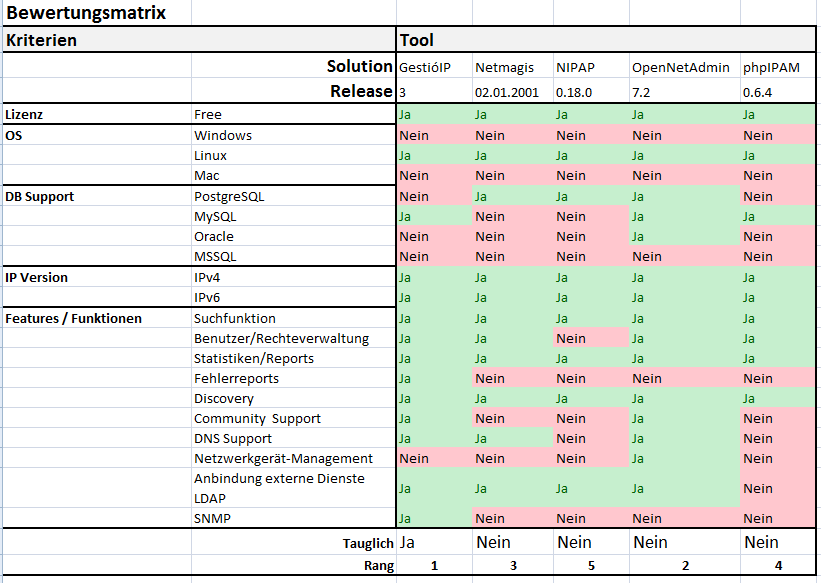
\includegraphics[width=0.8\textwidth]{Phase3/Matrix_1.png}
\caption{Bewertungsmatrix ausgefüllt mit Rangliste}
\label{fig:matrix_1}
\end{figure}

Da nicht alle Features und Funktionen gleich wichtig sind, haben wir für die verschiedenen Kriterien Punkte verteilt. Aufgrund der ausgefüllten Matrix konnten wir nun die in Abbildung \ref{fig:matrix_1} ersichtliche Rangliste der Tools erstellen.
\begin{figure}[H]
\centering
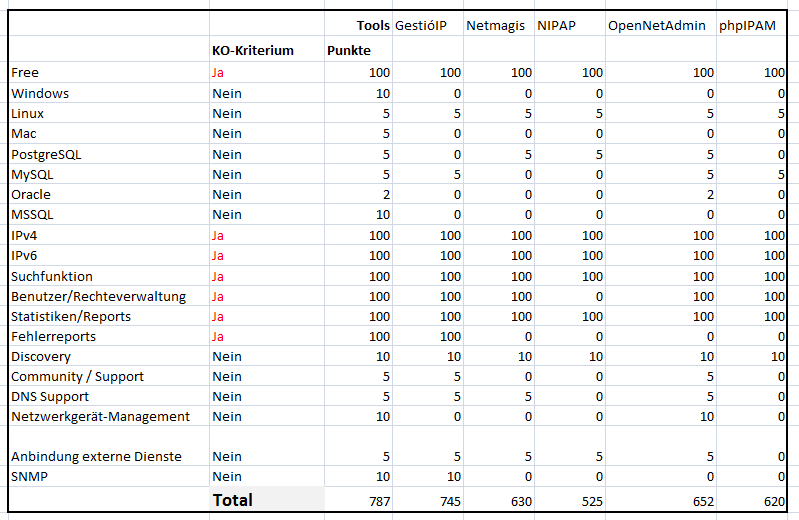
\includegraphics[width=0.8\textwidth]{Phase3/Matrix_2.png}
\caption{Bewertungsmatrix Punkteverteilung}
\label{fig:matrix_2}
\end{figure}

Die KO-Kriterien wurden mit 100 Punkte bewertet. Alle anderen Kriterien haben zusammen nicht mehr Gewicht als 100 Punkte. Tauglich sind nur jene Tools, welche mindestens 700 Punkte erreicht haben. In der Abbildung  \ref{fig:matrix_2} sind die KO-Kriterien ersichtlich, sowie die verteilung der Punkte und die effektiv erreichten Punkte.
\subsection{Implementation in Laborumgebung}
\subsubsection{Installation}
\subsubsection{Konfiguration}
\subsubsection{Reporting}
\subsubsection{Management}
\subsubsection{Fazit}
\textit{Optional}

\newpage
\appendix
\phantomsection
\addcontentsline{toc}{section}{Anhang}
\section{Konfiguration Core}
\lstinputlisting{core_config_labor.txt}
\newpage

\section{Konfiguration ASA}
\lstinputlisting{asa_config_labor.txt}
\newpage

\section{Konfiguration Switch}
\lstinputlisting{switch_config_labor.txt}
\newpage

\section{Tinc Startscript VMware}
\label{app:tinc-start-esx}
\lstinputlisting{tinc_ethernet_bridges/tinc_esx/start_bridges.sh}
\newpage

\section{Tinc Startscript Lab}
\label{app:tinc-start-lab}
\lstinputlisting{tinc_ethernet_bridges/tinc_lab/start_bridges.sh}
\newpage


\end{document}